\documentclass[12pt]{article}

\usepackage{answers}
\usepackage{setspace}
\usepackage{graphicx}
\usepackage{enumitem}
\usepackage{multicol}
\usepackage{mathrsfs}
\usepackage[margin=1in]{geometry} 
\usepackage{amsmath,amsthm,amssymb}
\usepackage{pgfplots}
\usepackage{listings}
\pgfplotsset{compat=1.15}
\usepgfplotslibrary{fillbetween}
 
\newcommand{\N}{\mathbb{N}}
\newcommand{\Z}{\mathbb{Z}}
\newcommand{\C}{\mathbb{C}}
\newcommand{\R}{\mathbb{R}}

\DeclareMathOperator{\sech}{sech}
\DeclareMathOperator{\csch}{csch}
 
\newenvironment{theorem}[2][Theorem]{\begin{trivlist}
\item[\hskip \labelsep {\bfseries #1}\hskip \labelsep {\bfseries #2.}]}{\end{trivlist}}
\newenvironment{definition}[2][Definition]{\begin{trivlist}
\item[\hskip \labelsep {\bfseries #1}\hskip \labelsep {\bfseries #2.}]}{\end{trivlist}}
\newenvironment{proposition}[2][Proposition]{\begin{trivlist}
\item[\hskip \labelsep {\bfseries #1}\hskip \labelsep {\bfseries #2.}]}{\end{trivlist}}
\newenvironment{lemma}[2][Lemma]{\begin{trivlist}
\item[\hskip \labelsep {\bfseries #1}\hskip \labelsep {\bfseries #2.}]}{\end{trivlist}}
\newenvironment{exercise}[2][Exercise]{\begin{trivlist}
\item[\hskip \labelsep {\bfseries #1}\hskip \labelsep {\bfseries #2.}]}{\end{trivlist}}
\newenvironment{solution}[2][Solution]{\begin{trivlist}
\item[\hskip \labelsep {\bfseries #1}]}{\end{trivlist}}
\newenvironment{problem}[2][Problem]{\begin{trivlist}
\item[\hskip \labelsep {\bfseries #1}\hskip \labelsep {\bfseries #2.}]}{\end{trivlist}}
\newenvironment{question}[2][Question]{\begin{trivlist}
\item[\hskip \labelsep {\bfseries #1}\hskip \labelsep {\bfseries #2.}]}{\end{trivlist}}
\newenvironment{corollary}[2][Corollary]{\begin{trivlist}
\item[\hskip \labelsep {\bfseries #1}\hskip \labelsep {\bfseries #2.}]}{\end{trivlist}}
 
\begin{document}
 
% --------------------------------------------------------------
%                         Start here
% --------------------------------------------------------------
 
\title{Problem Set 4}%replace with the appropriate homework number
\author{Basil R. Yap\\ %replace with your name
50.021 Artificial Intelligence - Term 8} %if necessary, replace with your course title
\date{June 12, 2018}
\maketitle
%Below is an example of the problem environment

\section{Theory Component}
% Question 1
\begin{figure}[h!]
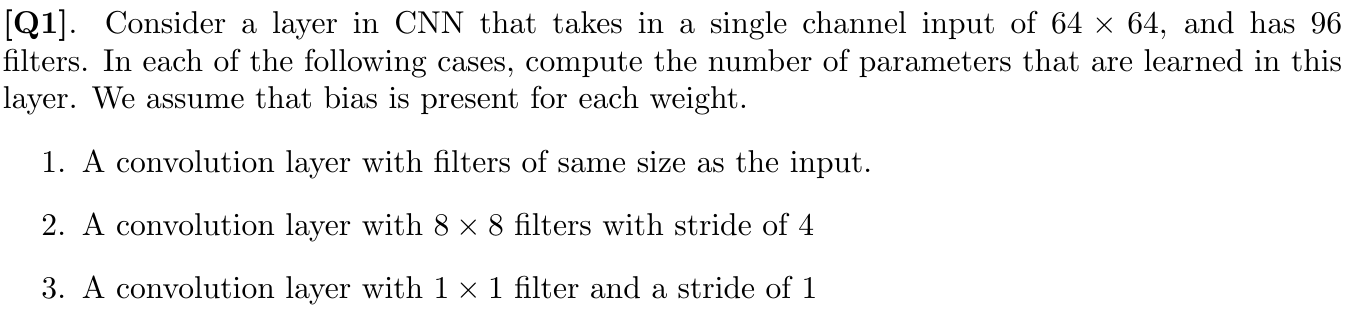
\includegraphics[width=\linewidth]{./assets/201806161634.png}
\end{figure}

\begin{solution}{}~
\begin{enumerate}
\item one convolution filter:\\
\begin{align*}
\text{no of parameters}&=\text{size of filter}\times\text{number of channels}+1\\
&=64\times64\times1+1\\
&=4097
\end{align*}

full convolution layer:\\
\begin{align*}
\text{no of parameters}&=4097\times96\\
&=393312
\end{align*}
number of parameters for one convolution filter:\\
\begin{align*}
\text{no of parameters}&=8\times8\times1+1\\
&=65
\end{align*}

full convolution layer:\\
\begin{align*}
\text{no of parameters}&=65\times96\\
&=6240
\end{align*}
\item one convolution filter:\\
\begin{align*}
\text{no of parameters}&=1\times1\times1+1\\
&=2
\end{align*}

full convolution layer:\\
\begin{align*}
\text{no of parameters}&=2\times96\\
&=192
\end{align*}
\end{enumerate}
\end{solution}

% Question 2
\begin{figure}[h!]
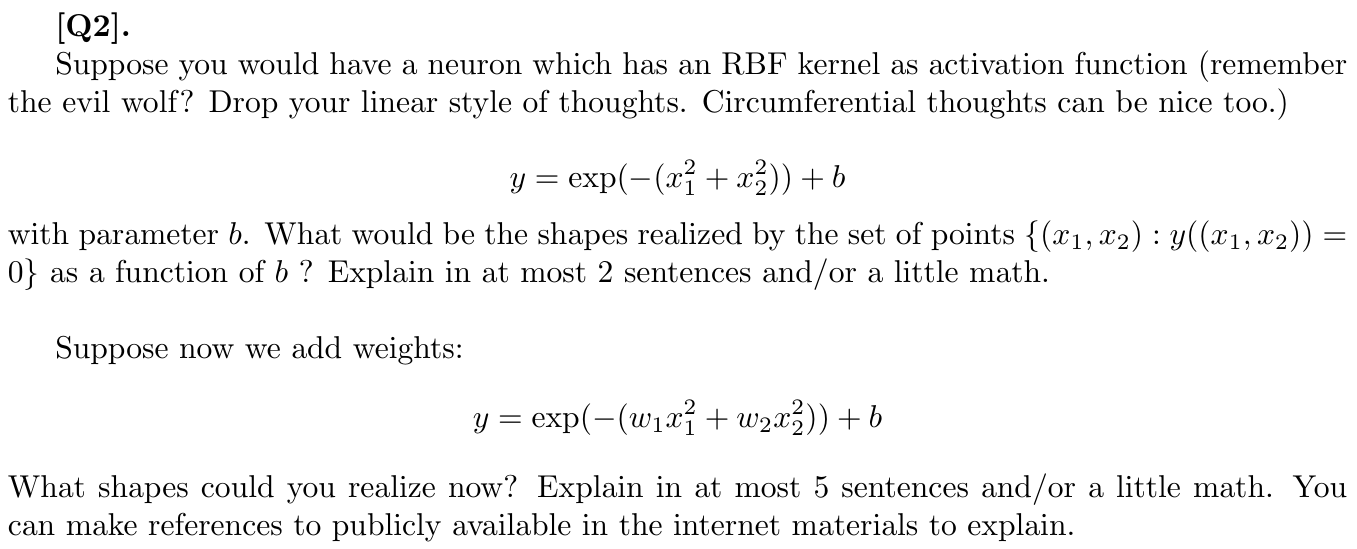
\includegraphics[width=\linewidth]{./assets/201806161635.png}
\end{figure}

\begin{solution}{}~
For $y=\exp(-(x_1^2+x_2^2))+b$, when $(x_1,x_2):y((x_1,x_2))=0$
\begin{align*}
0&=\exp(-(x_1^2+x_2^2))+b\\
-b&=\exp(-(x_1^2+x_2^2))\\
-\ln(-b)&=x_1^2+x_2^2\\
\end{align*}
The shape of the function is a circle with centre, $x_1=0,\ x_2=0$ and radius, $\sqrt{-\ln(-b)}$.\\
\begin{align*}
\sqrt{-\ln(-b)}&\geq0\\
-\ln(-b)&\geq0\\
\ln(-b)&\leq0
\end{align*}
$$
\begin{array}{rlrl}
-b\leq&\exp(0) & -b&\geq0\\
b&\geq-1 & b&\leq0\\
\end{array}
$$
\begin{center}
where $-1\geq b\geq0$
\end{center}

For $y=\exp(-(w_1x_1^2+w_2x_2^2))+b$, when $(x_1,x_2):y((x_1,x_2))=0$
\begin{align*}
0&=\exp(-(w_1x_1^2+w_2x_2^2))+b\\
-b&=\exp(-(w_1x_1^2+w_2x_2^2))\\
-\ln(-b)&=w_1x_1^2+w_2x_2^2\\
\frac{-\ln(-b)}{w_1w_2}&=\frac{x_1^2}{w_2}+\frac{x_2^2}{w_1}
\end{align*}
The shape of the function is a ellipse with centre, $x_1=0,\ x_2=0$,\\ $x_1$-axis radius, $\sqrt{\frac{-\ln(-b)}{w_1}}$ and $x_2$-axis radius, $\sqrt{\frac{-\ln(-b)}{w_2}}$.\\
where $-1\geq b\geq0$
\end{solution}

% Question 3
\begin{figure}[h!]
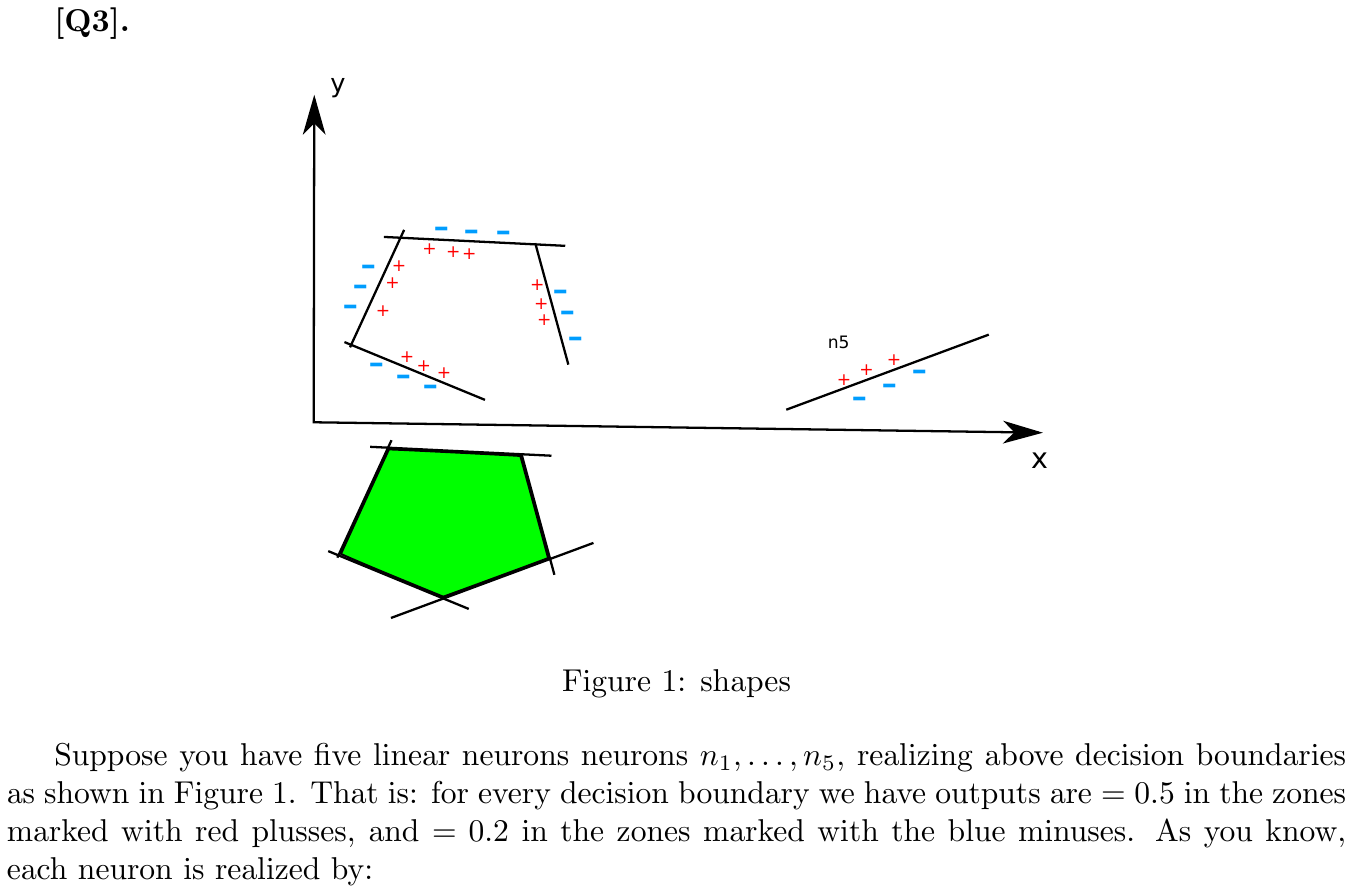
\includegraphics[width=\linewidth]{./assets/201806161636.png}
\end{figure}
\pagebreak
\begin{figure}[h!]
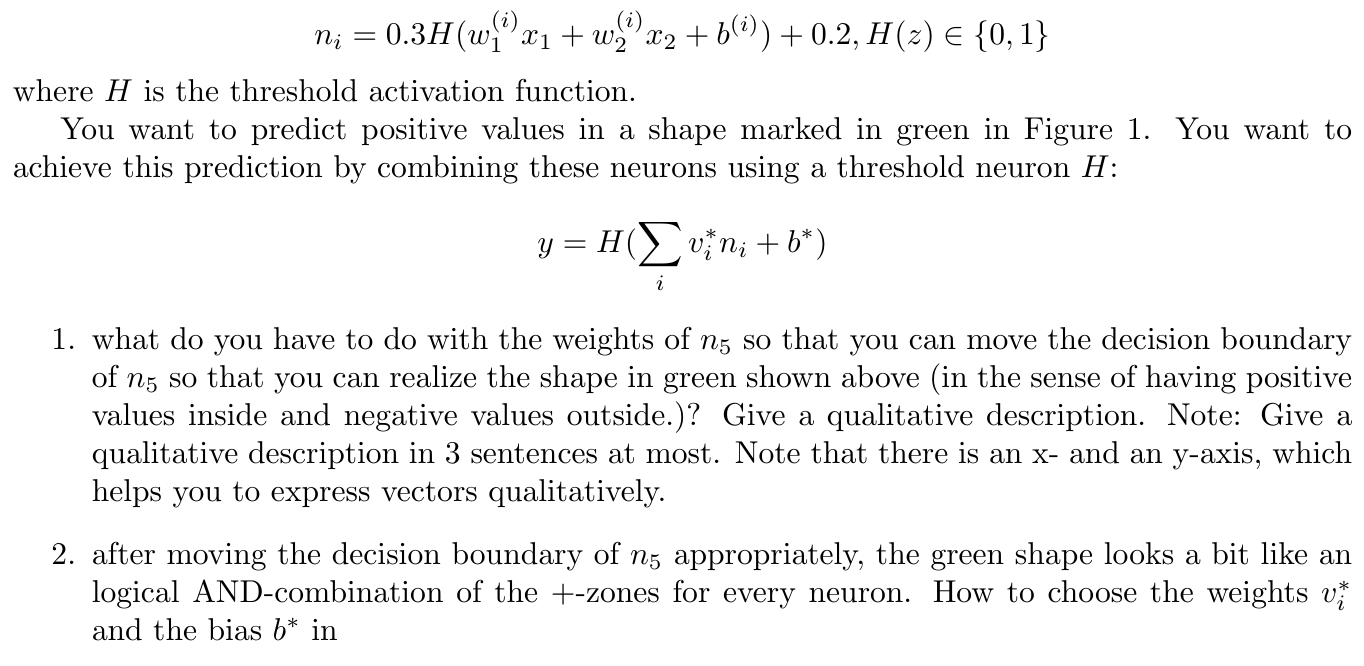
\includegraphics[width=\linewidth]{./assets/201806161708.png}
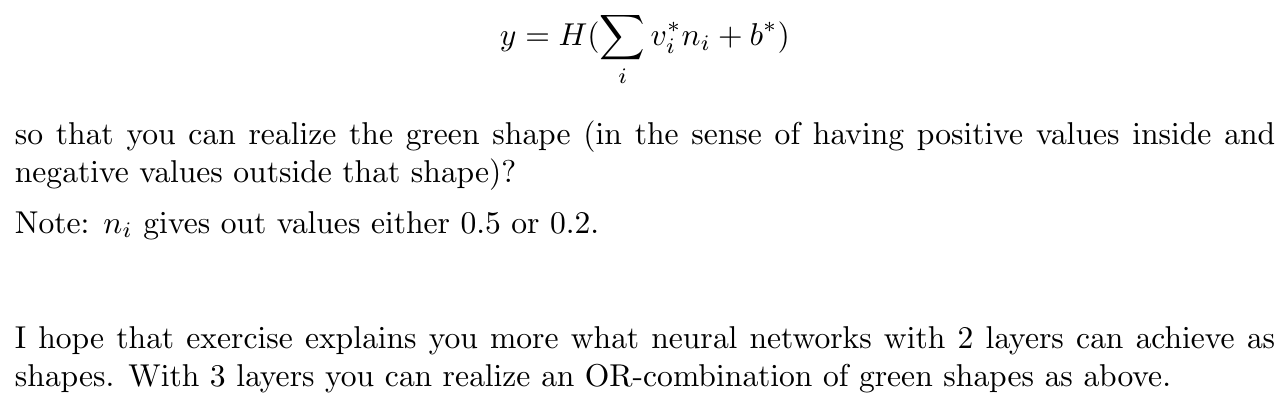
\includegraphics[width=\linewidth]{./assets/201806161709.png}
\end{figure}

\begin{solution}{}~
\begin{enumerate}
\item The decision boundary of $n_5$ is a linear function with gradients that is a function of the ratio of $w_1$ and $w_2$, and bias that is a function of the ratio of $b$ and $w_2$.\\
In order to shift the decision boundary, we need to decrease the value of $b$.
\item Let $H(x)=1[z>0]$\\
$$
\text{where }1[x]=\left\{\begin{array}{ll}
1 & \text{If }x\text{ is True}\\
0 & \text{If }x\text{ is False}
\end{array}\right.
$$

Consider when within the green region $y=1$ and $n_i=0.5$ $\forall i\in[1,n]$
\begin{align*}
1&=H(\sum_i0.5v_i^*+b^*)\\
1&=1[(\sum_i0.5v_i^*+b^*)>0]\\
\sum_i&0.5v_i^*+b^*>0\\
b^*&>-\sum_i0.5v_i^*
\end{align*}

Consider when outside the green region $y=0$, $n_j=0.2$ and $n_i=0.5$ $\forall i\in([1,n]\setminus j)$
\begin{align*}
0&=H(\sum_{i}0.5v_i^*+0.2v_j^*+b^*)\\
0&=1[(\sum_i0.5v_i^*+0.2v_j^*+b^*)>0]\\
\sum_i&0.5v_i^*+0.2v_j^*+b^*\leq0\\
\sum_i&0.5v_i^*+0.2v_j^*+b^*\leq0\\
b^*&\leq-\sum_i0.5v_i^*-0.2v_j^*\\
-\sum_i&0.5v_i^*-0.5v_j^*<b^*\leq-\sum_i0.5v_i^*-0.2v_j^*
\end{align*}

We can get the bounded green region as long as we satisfy the above inequality for all values of $v_k$ $\forall k\in[1,n]$ with all combinations $\forall j\in[1,n]$ with $i\in([1,n]\setminus j)$.
\end{enumerate}
\end{solution}

\pagebreak

\section{Coding Component}

\lstinputlisting[language=Python]{pset4.py}

\end{document}
